\documentclass[9pt,english,twoside,openright]{scrbook}
\usepackage{style/header}
%SYMBOLS
\def\minus{%
  \setbox0=\hbox{-}%
  \vcenter{%
    \hrule width\wd0 height \the\fontdimen8\textfont3%
  }%
}

\newcommand{\rmplus}{\ensuremath{+}}
\newcommand{\rmminus}{\ensuremath{\raisebox{0.1pt}{\scalebox{0.6}[0.75]{$-$}}}}

\newcommand{\range}{\ensuremath{\text{--}}}
\newcommand{\scriptn}[1]{\mathalpha{\raisebox{0.0pt}[0pt][0pt]{$\scriptstyle#1$}}}


% PROCESSES
\newcommand{\qcd}{\ensuremath{QCD}\xspace}
\newcommand{\wjets}{\ensuremath{\textrm{W\mbox{+}jets}}\xspace}
\newcommand{\zjets}{\ensuremath{\textrm{$Z/\gamma^*$\mbox{+}jets}}\xspace}
\newcommand{\vjets}{\ensuremath{\textrm{V\mbox{+}jets}}\xspace}
\newcommand{\ttbar}{\ensuremath{\mathrm{t}\bar{\mathrm{t}}}\xspace}
\newcommand{\tw}{\ensuremath{\mathrm{tW}}\xspace}
\newcommand{\tch}{\ensuremath{t\mathrm{\mbox{-}channel}}\xspace}


% VARIABLES
\newcommand{\pt}{\ensuremath{p_\mathrm{T}}\xspace}
\newcommand{\muiso}{\ensuremath{I_\mathrm{rel.}^{\mu}}\xspace}
\newcommand{\eiso}{\ensuremath{I_\mathrm{rel.}^{e}}\xspace}
\newcommand{\mtop}{\ensuremath{m_{\mu\nu \mathrm{b}}}\xspace}
\newcommand{\mw}{\ensuremath{m_{\mathrm{W}}}\xspace}
\newcommand{\met}{\ensuremath{\slashed{E}_{\mathrm{T}}}\xspace}
\newcommand{\mtw}{\ensuremath{m_{\mathrm{T}}(\mathrm{W})}\xspace}
\newcommand{\pvmiss}{\ensuremath{\vec{\slashed{p}}_\mathrm{T}}\xspace}
\newcommand{\pvmissx}{\ensuremath{\slashed{p}_{x}}\xspace}
\newcommand{\pvmissy}{\ensuremath{\slashed{p}_{y}}\xspace}
\newcommand{\pvmissz}{\ensuremath{\slashed{p}_{z}}\xspace}
\newcommand{\bdt}{\ensuremath{\mathrm{BDT}}\xspace}

\newcommand{\aem}{\ensuremath{{\alpha_\mathrm{EM}}}\xspace}
\newcommand{\aw}{\ensuremath{{\alpha_\mathrm{W}}}\xspace}
\newcommand{\as}{\ensuremath{{\alpha_\mathrm{s}}}\xspace}

\newcommand{\vtb}{\ensuremath{{\mathrm{V}_\mathrm{tb}}}\xspace}
\newcommand{\vts}{\ensuremath{{\mathrm{V}_\mathrm{ts}}}\xspace}
\newcommand{\vtd}{\ensuremath{{\mathrm{V}_\mathrm{td}}}\xspace}

%UNITS
\newcommand{\eV}{\ensuremath{\mathrm{eV}}\xspace}
\newcommand{\keV}{\ensuremath{\mathrm{keV}}\xspace}
\newcommand{\MeV}{\ensuremath{\mathrm{MeV}}\xspace}
\newcommand{\GeV}{\ensuremath{\mathrm{GeV}}\xspace}
\newcommand{\TeV}{\ensuremath{\mathrm{TeV}}\xspace}

\newcommand{\pb}{\ensuremath{\mathrm{pb}}\xspace}
\newcommand{\fb}{\ensuremath{\mathrm{fb}}\xspace}
\newcommand{\ab}{\ensuremath{\mathrm{ab}}\xspace}

\newcommand{\pbinv}{\ensuremath{\mathrm{pb}^{-1}}\xspace}
\newcommand{\fbinv}{\ensuremath{\mathrm{fb}^{-1}}\xspace}
\newcommand{\abinv}{\ensuremath{\mathrm{ab}^{-1}}\xspace}

%PARTICLES
\newcommand{\photon}{\ensuremath{{\gamma}}\xspace}
\newcommand{\zboson}{\ensuremath{{\mathrm{Z}^{0}}}\xspace}
\newcommand{\wboson}{\ensuremath{{\mathrm{W}^{\pm}}}\xspace}
\newcommand{\higgs}{\ensuremath{{\mathrm{H}^{0}}}\xspace}



% FORMATTING
\newcommand{\typew}[1]{\texttt{\detokenize{#1}}}
\newcount\colveccount
\newcommand*\colvec[1]{
    \global\colveccount#1
    \begin{pmatrix}
    \colvecnext
}
\def\colvecnext#1{
    #1
    \global\advance\colveccount-1
    \ifnum\colveccount>0
        \\
        \expandafter\colvecnext
    \else
        \end{pmatrix}
    \fi
}

% OTHER
\newcommand{\msbar}{\ensuremath{\overline{\text{MS}}}\xspace}

\newcommand{\invfb}{\ensuremath{\mathrm{fb}^{-1}}\xspace}
\newcommand{\invpb}{\ensuremath{\mathrm{pb}^{-1}}\xspace}
\newcommand{\jprime}{\ensuremath{j^{\prime}}\xspace}
\newcommand{\qprime}{\ensuremath{q^{\prime}}\xspace}
\newcommand{\bjtop}{\ensuremath{j_\mathrm{b,top}}\xspace}

\newcommand{\HATHOR}{\texttt{HATHOR}\xspace}
\newcommand{\POWHEG}{\texttt{POWHEG}\xspace}
\newcommand{\MG}{\texttt{MadGraph}5\xspace}
\newcommand{\AMC}{a\texttt{MC@NLO}\xspace}
\newcommand{\MGAMC}{\texttt{MadGraph}5\_a\texttt{MC@NLO}\xspace}
\newcommand{\COMPHEP}{\texttt{CompHEP}\xspace}
\newcommand{\PYTHIA}{\texttt{Pythia}\xspace}
\newcommand{\HERWIG}{\texttt{Herwig}\xspace}
\newcommand{\tunfold}{\texttt{TUnfold}\xspace}

%\def\todolist{\subsection{TODO list}}
%\newcommand{\addtodolist}[1]{\expandafter\def\expandafter\todolist\expandafter{\todolist{}\\ #1}}
%\newcommand{\todo}[1]{\textsc{\color{red}{\textbf{TODO}: #1}}\addtodolist{#1}}
%\newcommand{\todo}[1]{}

\loadglsentries{sections/acronyms}

\begin{document}
\setupTextStyle

%\begin{clearedpagestyle}

\vspace*{0.5cm}

\parbox[c][][c]{0.2\textwidth}{
\includegraphics[height=2.cm]{figures/title/UCL.pdf}
}\parbox[c][][c]{0.7\textwidth}{\vspace{0.05cm}\small
Universit{\'e} catholique de Louvain\\[0.1cm]
\footnotesize Secteur des Sciences et Technologies\\ 
Institut de Recherche en Math{\'e}matique et Physique\\ 
Center for Cosmology, Particle Physics and Phenomenology
}

\vspace{1.0cm}

\begin{center}
{\rule{\textwidth}{\myrulewidth}}

\vspace{0.15cm}

\parbox{0.95\textwidth}{
\numberfont\fontsize{16}{22}\selectfont\centering
Measurements of differential t-channel single-top-quark production cross sections at 8~and 13~TeV with the CMS experiment\\
and\\
Emulation of track reconstruction within the CMS simulation software
}

\vspace{0.15cm}

{\rule{\textwidth}{\myrulewidth}}
\end{center}
\vspace{0.4cm}

\begin{center}
Doctoral dissertation presented by \\
\vspace{3mm}
{\numberfont\fontsize{14}{14}\selectfont Matthias Komm}\\
\vspace{3mm}
in fulfilment of the requirements for the degree of Doctor in Sciences
\end{center}

\vspace{\fill}

\begin{center}
\begin{tabular*}{0.8\textwidth}{l @{\extracolsep{\fill}} r}
\fontsize{12}{12}\selectfont Thesis support committee & \\[2pt]
{\numberfont Prof. Andrea Giammanco} \sl (Advisor) & UCL, Belgium \\
{\numberfont Prof. Giacomo Bruno} & UCL, Belgium \\
{\numberfont Prof. Freya Blekman} & VUB, Belgium \\
\end{tabular*}

\vspace*{0.5cm}
{\color{gray}\rule{0.3\textwidth}{\myrulewidth}}\\[1pt]
\textsl{May, 2017}\\[1pt]

\end{center}
\cleardoublepage
\end{clearedpagestyle}


%\cleardoublepage


\microtypesetup{protrusion=false}
\tableofcontents
\microtypesetup{protrusion=true}
\cleardoublepage

%\chapter{Introduction of the}

\lipsum[1]

\begin{align}
\sqrt{7\,TeV} & =100\,{GeV}
\end{align}


\lipsum[4]

\lipsum[2]

\lipsum[1] 7\,GeV = 100\,GeV.

\begin{equation}
\sqrt{7\,TeV}=100\,{GeV}+\mathrm{GeV}+\sum_{i}\sqrt{\frac{\Big(\nabla\mathcal{A}+\xi\mathfrak{B}-\vec{x}^{2}\Big)_{i}^{\dagger}}{x-y^{3}}}
\end{equation}


\lipsum[4]


\section{Reconstruction}


\subsection{Reconstruction}

\lipsum[2]

\lipsum[1]


\chapter{Introduction of the CMS x x detector and the $\phi$-system hu hu}

\lipsum[4]

\lipsum[2]

\lipsum[2]

\lipsum[1]

\lipsum[2]

\begin{table}[th]
\caption{This is a table. This is a table. This is a table. This is a table.
This is a table. This is a table. This is a table. This is a table.}


\centering{}%
\begin{tabular}{|c|c|c|c|c|}
\hline 
 &  &  &  & \tabularnewline
\hline 
\hline 
 &  &  &  & \tabularnewline
\hline 
 &  &  &  & \tabularnewline
\hline 
 &  &  &  & \tabularnewline
\hline 
 &  &  &  & \tabularnewline
\hline 
\end{tabular}
\end{table}


\lipsum[1]bla blu blub\footnote{\lipsum[1]}. Bla blu blub.\lipsum[1]

\lipsum[2]

\lipsum[1]bla blu blub\footnote{bla blu blub.}. bla blu blub\footnote{bla blu blub.}. bla blu blub\footnote{bla blu blub.}. Bla blu blub.\lipsum[1]

\lipsum[2]


\section{Reconstruction tector and the $\phi$-system hu hu}

\lipsum[4]


\section{Reconstruction}

\lipsum[2]


\subsubsection{test test}

\lipsum[1]

\begin{equation}
\sqrt{7\,TeV}=100\,{\ GeV}
\end{equation}


\lipsum[4]

\lipsum[2]
\begin{figure}[th]
\begin{center}
\missingfigure[figwidth=6cm]{Testing a long text string}
\end{center}

\caption{Test Figure. Test Figure. Test Figure. Test Figure. Test Figure. Test
Figure. Test Figure. Test Figure. Test Figure. Test Figure. Test Figure.
Test Figure. Test Figure. Test Figure. Test Figure. Test Figure. Test
Figure. Test Figure. Test Figure. Test Figure. Test Figure.}
\end{figure}


\lipsum[1]

\begin{equation}
\sqrt{7\,TeV}=100\,{\ GeV}
\end{equation}


\lipsum[4]

\lipsum[2]

\begin{figure}[th]
\begin{center}
\missingfigure[figwidth=6cm]{Testing a long text string}
\end{center}

\caption{Test Figure. Test Figure. Test Figure. Test Figure. Test Figure. Test
Figure. Test Figure. Test Figure. Test Figure. Test Figure. Test Figure.
Test Figure. Test Figure. Test Figure. Test Figure. Test Figure. Test
Figure. Test Figure. Test Figure. Test Figure. Test Figure.}
\end{figure}


\lipsum[4]


\subsection{Reconstruction}

\lipsum[1]

\begin{equation}
\sqrt{7\,TeV}=100\,{\ GeV}
\end{equation}


\lipsum[4]

\cleardoublepage
\renewcommand{\chaptername}{Appendix}
\renewcommand\thechapter{\Alph{chapter}}
\setcounter{chapter}{0}
\addcontentsline{toc}{chapter}{\chaptername}

\appendixchapter{Additional Material}

\lipsum[2]

\appendixchapter{Some plots}

\lipsum[2]

\cleardoublepage
%\pagenumbering{Alph}
%\setcounter{page}{1}




\lipsum[4]

\lipsum[2]

\begin{itemize}
\item \lipsum[1]
\item Test item
\item \lipsum[2]
\end{itemize}

\lipsum[4]

\begin{enumerate}
\item \lipsum[1]
\item blublu blu b blue \texttt{Test item} quark quark
\item \lipsum[2]
\end{enumerate}

\lipsum[2]

\begin{figure}[th]
\begin{center}
\missingfigure[figwidth=6cm]{Testing a long text string}
\end{center}

\caption{Test Figure. Test Figure. Test Figure. Test Figure. Test Figure. Test
Figure. Test Figure. Test Figure. Test Figure. Test Figure. Test Figure.
Test Figure. Test Figure. Test Figure. Test Figure. Test Figure. Test
Figure. Test Figure. Test Figure. Test Figure. Test Figure.}
\end{figure}


\lipsum[2]

\lipsum[2]

\begin{figure}[th]
\begin{center}
\missingfigure[figwidth=6cm]{Testing a long text string}
\end{center}

\caption{Test Figure. Test Figure. Test Figure. Test Figure. Test Figure. Test
Figure. Test Figure. Test Figure. Test Figure. Test Figure. Test Figure.
Test Figure. Test Figure. Test Figure. Test Figure. Test Figure. Test
Figure. Test Figure. Test Figure. Test Figure. Test Figure.}
\end{figure}


\lipsum[2]

\lipsum[2]

\begin{figure}[th]
\begin{center}
\missingfigure[figwidth=6cm]{Testing a long text string}
\end{center}

\caption{Test Figure. Test Figure. Test Figure. Test Figure. Test Figure. Test
Figure. Test Figure. Test Figure. Test Figure. Test Figure. Test Figure.
Test Figure. Test Figure. Test Figure. Test Figure. Test Figure. Test
Figure. Test Figure. Test Figure. Test Figure. Test Figure.}
\end{figure}


\lipsum[2]

\begin{figure}[th]
\begin{center}
\missingfigure[figwidth=6cm]{Testing a long text string}
\end{center}

\caption{Test Figure. Test Figure. Test Figure. Test Figure. Test Figure. Test
Figure. Test Figure. Test Figure. Test Figure. Test Figure. Test Figure.
Test Figure. Test Figure. Test Figure. Test Figure. Test Figure. Test
Figure. Test Figure. Test Figure. Test Figure. Test Figure.}
\end{figure}


\lipsum[2]




%\chapter*{Introduction}
\addcontentsline{toc}{chapter}{Introduction}

The \acrlong{sm} is a very successful theory in describing electroweak and strong interactions between fundamental particles. Its predictions are constantly challenged with experimental data but so far no significant deviations have been confirmed. 

The heaviest known elementary particle is the top quark whose mass is similar to a gold atom. It has been discovered in 1995 by the \gls{cdf} and \gls{d0} experiments at the Tevatron (Fermilab, USA) through its production process via strong interactions leading to top quark/antiquark pairs. An experimentally more elusive production mode of top quarks predicted by the standard model occurs via electroweak interactions resulting into events containing only single top quarks. The detection of such events is more challenging due to the larger occurrence of background events mimicking its signature. It took 14 more years until the production of single top quarks was finally observed as well in 2009 by the \gls{cdf} and \gls{d0} experiments. With the start of the physics program at the \gls{lhc} (\gls{cern}, Switzerland) in 2009, the production of single top quarks can be studied for the first time in great detail utilizing an unprecedented quantity of proton-proton collision events.

Single top quark events offer an unique opportunity to measure the properties of the electroweak theory and to test its predictions in the presence of such a heavy particle. For instance, measurements of the inclusive cross section of single-top-quark production allow to infer the modulus of the \gls{ckm} matrix element $\vtb$ whose value is not predicted by the standard model. Measurements of differential cross section on the other hand allow to perform in-deep tests of the electroweak production mechanisms.

In this thesis, the production of single top quarks via $t$~channel is investigated.  First measurements of differential cross sections at \acrlong{cm} energies of 8 and 13~\TeV, based on data recorded with the \gls{cms} experiment, are presented. 

In 8~\TeV data, the top quark polarization angle is studied which is defined between the lepton from the top quark decay and the spectator quark in the top quark rest frame. The top quark spin asymmetry, a quantity related to the top quark polarization, is extracted from its differential cross section. The asymmetry allows to test the coupling structure of the involved electroweak interaction. In the standard model, a \gls{va} coupling structure is predicted which permits only left-handed top quarks or right-handed top antiquarks to interact with a W~boson and a bottom quark. One expects therefore that single top quarks in $t$~channel are produced highly polarized. However, a potential depolarization may occur through new physics models beyond the standard model. In an effective approach their influence can be recast into anomalous couplings for which limits are derived using the measured spin asymmetry.

In the second part, an early measurement of differential cross sections as a function of the top quark transverse momentum and rapidity is presented using the first data recorded at a \acrlong{cm} energy of 13~\TeV with the \gls{cms} experiment in 2015. For this, the analysis strategy of the top quark polarization measurement has been significantly extended which resulted into various benefits. The measured cross sections are compared to the predictions of the single-top-quark spectra by various event generator programs.

The thesis is organized as follows. First a general introduction to the standard model is given in Ch.~\ref{ch:theory}. The phenomenology of top quark properties and its production mechanisms, relevant for this thesis, are introduced in Ch.~\ref{ch:top} with a particular emphasis on the electroweak coupling structure. The experimental setup consisting of the \gls{lhc} accelerator and the \gls{cms} experiment is outlined in Ch.~\ref{ch:exp} which is followed by a detailed description of the reconstruction of physics objects for analyses in Ch.~\ref{ch:exp}. In Ch.~\ref{ch:technique} the analysis techniques are elaborated. The differential cross section measurements at 8 and 13~\TeV are detailed in Ch.~\ref{ch:polarization} and Ch.~\ref{ch:diff13} respectively. Potential prospects on a future measurement have been studied in Ch.~\ref{ch:prospects}. The thesis is concluded in Ch.~\ref{ch:conclusion}.

In addition, an introduction to the emulation of track reconstruction in the fast simulation package of \gls{cms} can be found in the appendix (App.~\ref{ch:fsim}).

\section*{Unit convention}
\addcontentsline{toc}{section}{Unit convention}

The ``natural units'' of particle physics\footnote{Other fields of physics can have their own ``natural units'' which may not coincide with the definition used here.} are used throughout this thesis unless it is explicitly stated otherwise. These differ from the \glsmark{si} units and are derived by defining the natural constants as:

\begin{itemize}
\item speed of light: $\mathrm{c}\equiv 1$\,;
\item Planck constant: $\hbar\equiv 1$\,;
\item electric permittivity: $\epsilon_{0}\equiv 1$\,;
\item Boltzmann constant: $k_\mathrm{B}\equiv 1$\,.
\end{itemize}

This changes the units of the following quantities amongst others:

\begin{itemize}
\item length: $\big[\mathrm{m}\big]\rightarrow \big[\eV^{-1}\big]$\,;
\item time: $\big[\mathrm{s}\big]\rightarrow \big[\eV^{-1}\big]$\,;
\item mass: $\big[\mathrm{kg}\big]\rightarrow \big[\eV\big]$\,;
\item energy: $\big[\mathrm{J}\big]\rightarrow \big[\eV\big]$\,;
\item temperature: $\big[\mathrm{K}\big]\rightarrow \big[\eV\big]$\,.
\end{itemize}




%\chapter{Theory and experimental status}

An introduction to the \gls{sm}, its particle content, interactions, and properties is provided in the following. Special focus is attributed to the top quark which is the heaviest known fundamental particle to date. Here, latest experimental results are discussed and the theoretical foundation of the measurements within this thesis is laid out.


\section{General Quantum Field Theory of the Standard Model}

The \gls{sm} describes the interactions between fundamental particles. It is based on \gls{qft} which allows to predict observables of particle interactions. Exemplary observables are production cross sections or lifetimes of unstable particles which can be calculated within its framework -- even fully automatized. The \gls{sm} validity is constantly challenged by comparing predictions to experimental data. No significant deviations have been found so far that would hint towards physics \gls{bsm}.


\subsection{Particle content}

Fundamental particles are objects for which experiments have revealed no internal structure. For example, the spatial radius of an electron has been limited to be smaller than $<10^{-18}~\mathrm{m}$~\cite{PhysRevLett.97.030801}. Such particles are therefore considered as point-like. Fundamental particles can be grouped by their spin into fermions with spin~$\frac{1}{2}$ and bosons with integer spin. The fermions can be further divided into leptons and quarks where only the later can participate in strong interactions. Tables~\ref{tab:theory-leptons} and~\ref{tab:theory-quarks} list the leptons and quarks respectively. Each column encapsulating an isospin pair~(up/down) of fermions is called a generation. It is unknown why there are exactly three lepton and three quark generations.

\mytable{\label{tab:theory-leptons}Leptons of the \gls{sm}. Particle masses are taken from Ref.~\cite{Olive:2016xmw}. Only \glspl{cl} are given for the neutrino masses.}{
\begin{tabular}{r||c|c|c}
                    & 1. generation                  & 2. generation                  & 3. generation \\
\hline
\hline
name                & electron (e)                  & muon ($\mu$)                  & tau ($\tau$) \\
\hline
mass                & $511.0~\keV$                  & $105.66~\MeV$                 & $1.776~\GeV$ \\
\hline
electric charge     & $-1$                          & $-1$                          & $-1$ \\
\hline
isospin (\isoz)     & $\frac{1}{2}$                 & $\frac{1}{2}$                 & $\frac{1}{2}$ \\
\hline
\hline
name                & electron neutrino             & muon neutrino                 & tau neutrino  \\
                    & ($\nu_{e}$)                   & ($\nu_{\mu}$)                 & ($\nu_{\tau}$) \\
\hline
mass                & $<225~\eV$                    & $<0.19~\MeV$                  & $<18.2~\MeV$ \\
                    & (95\% CL)                     & (90\% CL)                     & (95\%~CL)\\
\hline
electric charge     & 0                             & 0                             & 0 \\
\hline
isospin (\isoz)     & $-\frac{1}{2}$                & $-\frac{1}{2}$                & $-\frac{1}{2}$ \\
\end{tabular}
}

\mytable{\label{tab:theory-quarks}Quarks of the \gls{sm}.}{
\begin{tabular}{|c|c|c|c|c|}
\hline
\end{tabular}
}

For the neutrinos, only limits on


The bosons are connected to fundamental interactions and act as their mediators as explained later~(Secs.~\ref{sec:theory-ewk} and~\ref{sec:theory-qcd}). They are listed in Tab.~\ref{tab:theory-bosons}. The Higgs boson is the only scalar particle~(spin~$0$) of the \gls{sm}. All other bosons carry a spin of~$1$.


\mytable{\label{tab:theory-bosons}Bosons of the \gls{sm}.}{
\begin{tabular}{|c|c|c|c|c|}
\hline
\end{tabular}
}


Antiparticles


\subsection{General properties}
quantum fields, EW construction, gauge groups, symmetries, Noether currents, renormalization, running couplings
\subsection{Electroweak interactions}
\label{sec:theory-ewk}
chirality
\subsection{Higgs mechanism}
potential, CKM
\subsection{Strong interactions}
\label{sec:theory-qcd}
self-couplings, running coupling, nlo calculations
\subsection{Observables}
matrix elements, cross sections, decays, PDFs, angles (w polarizations)
\subsection{Open questions}
naturalness, gravity, gut, susy, dark matter

\section{The top quark}
\subsection{}

\chapter{Experimental setup}

\section{Large Hadron Collider}

\subsection{Accelerator complex}

\subsection{Experiments}

\section{CMS experiment}

\subsection{Magnet}

\subsection{Tracker}

\subsection{Electromagnetic calorimeter}

\subsection{Hadronic calorimeter}

\subsection{Muon systems}
DT/RPC/CSC

\subsection{Data acquisition}
Trigger/DAQ

\subsection{Operations}
DCS/DSS

%\chapter{Reconstruction of physics objects}

%\input{sections/simulation}
%\chapter{Methodology of analyses techniques}
%\chapter{Polarization of single top quarks in \textsl{t}~channel at 8~TeV}

\intro{A first measurement of the top quark spin asymmetry in t~channel, related to the top quark polarization, is presented in this chapter. Proton-proton collision data at $\mathit{\sqrt{s}=8}$~TeV have been analyzed corresponding to about $\mathit{20~fb^{-1}}$. Events with an isolated muon are selected together with two or three jets for the final measurement while events containing an isolated electron and jets have been studied as well. The normalized differential cross section is measured as a function of the polarization angle. From its shape, a spin asymmetry of $\mathit{0.26\pm0.03~(stat)\pm0.10~(syst)}$ is obtained. This is found to be compatible within $\mathit{2.0}$ standard deviations with the expected \gls{sm} asymmetry of $\mathit{0.44}$. The result has been published in Ref.~\cite{Khachatryan:2015dzz}. In a further step, the derivation of limits on anomalous couplings is illustrated by combining this measurement with related ones.}

The strategy to measure the top quark spin asymmetry is as follows. After event selection, two \glspl{bdt} are trained. The first one is optimized to reject events with fake leptons stemming from multijet production. The second \gls{bdt} is then trained to separate signal from \wjets and \ttbar events. 

\myfigure{}{
\subfloat[]{\adjincludegraphics[height=4.8cm,trim={0 0 {0.23\width} 0},clip]{figures/polarization/2j1t/muon_2j1t_met_qcdnone_nol.pdf}}
\hspace{0.017\textwidth}
\subfloat[]{\adjincludegraphics[height=4.8cm]{figures/polarization/2j1t/muon_2j1t_top_logmass_qcdnone.pdf}}\\
\subfloat[]{\adjincludegraphics[height=4.8cm,trim={0 0 {0.23\width} 0},clip]{figures/polarization/2j1t/muon_2j1t_mtw_qcdnone_nol.pdf}}
\hspace{0.017\textwidth}
\subfloat[]{\adjincludegraphics[height=4.8cm]{figures/polarization/2j1t/muon_2j1t_ljet_pt_qcdnone.pdf}}\\
\subfloat[]{\adjincludegraphics[height=4.8cm,trim={0 0 {0.23\width} 0},clip]{figures/polarization/2j1t/muon_2j1t_isotropy_qcdnone_nol.pdf}}
\hspace{0.017\textwidth}
\subfloat[]{\adjincludegraphics[height=4.8cm]{figures/polarization/2j1t/muon_2j1t_bdt_qcd_qcdnone.pdf}}
}


\section{Simulated samples and event selection}

separating, W+HF, W+LF
categorization (2j0t,2j1t,...)

\myfigure{\label{fig:polarization-categorization}Categorization of events depending on number of selected jets, number of b-tags, and the signal \gls{bdt} discriminant.}{
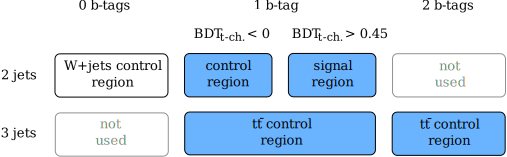
\includegraphics[scale=0.75]{figures/polarization/regions.pdf}
}

\section{Training of Boosted Decision Trees}


%choice of variables, correlation tests

\section{Signal extraction}

\section{W+jet modeling}

\section{Validation}

cosTheta, cosWhel, top mass in SR/CR, 2j0t,3j1t

\section{Unfolding}

bdt cut, neyman construction

\section{Statistical evaluation}

Q-scale reweighting, chi2 fit

\section{Results}

\myfigure{}{
\subfloat[]{\includegraphics[width=0.48\textwidth]{figures/polarization/result/unfolded_mu_top.pdf}}
\hspace{0.02\textwidth}
\subfloat[]{\includegraphics[width=0.48\textwidth]{figures/polarization/result/unfolded_mu_antitop.pdf}}\\
\subfloat[]{\includegraphics[width=0.48\textwidth]{figures/polarization/result/unfolded_mu.pdf}}
}

\section{Limits on anomalous couplings}

topfit
%\chapter{Differential single-top-quark cross sections at 13~TeV}

\section{BDT training}
\label{sec:diff13-bdt}
%\chapter{Conclusion}
\label{ch:conclusion}

polarization:
wp optimization, 2bin unfolding, q scale
eft limits

differential:
extended fitting

\glsaddall[types={acronym}] 
\printglossary[type=\acronymtype,title={Abbreviations},nonumberlist]
\cleardoublepage

%\nocite{*}
\bibliographystyle{style/bibstyle}
\renewcommand{\bibname}{References}
\bibliography{sections/references}

\todototoc
\listoftodos

\end{document}
